\chapter{Introducción}
Este proyecto tiene como objetivo la producción de una aplicación de realidad virtual de uso recreativo y, principalmente, didáctico, en la que esculpir a partir de un bloque macizo con el uso de distintas herramientas.

Con este propósito, se ha usado el motor gráfico Unreal principalmente debido a las herramientas que ofrece, muy avanzadas respecto a otros motores como Unity (con el que en un principio iba a realizarse este proyecto) y que permiten el desarrollo de aplicaciones en realidad virtual con una interacción mucho más compleja y precisa.

A continuación, antes de entrar a fondo en el desarrollo del proyecto, se explicará la motivación detrás de este, además de algunos conceptos base.

\section{Realidad virtual}

\subsection{Usos}

La realidad virtual, comúnmente conocida como VR (\textit{Virtual Reality}) es el campo de la informática gráfica que estudia la presentación e interacción con el usuario de tal forma que este se sienta trasladado a, como el nombre indica, otra realidad. \cite{wohlgenannt2020virtual} Esto tiene diversos usos, siendo el más famoso y expandido el entretenimiento, con videojuegos y otras aplicaciones de uso recreativo, como vídeos y presentaciones.

Sin embargo, otro uso menos famoso pero igualmente expandido es el de \textbf{entrenamiento}, como se puede ver en campos como la medicina, la aviación, el ejército, etcétera \cite{vrtraining} (Figura \ref{fig:vr_military}).

\begin{figure}[H]
	\centering
	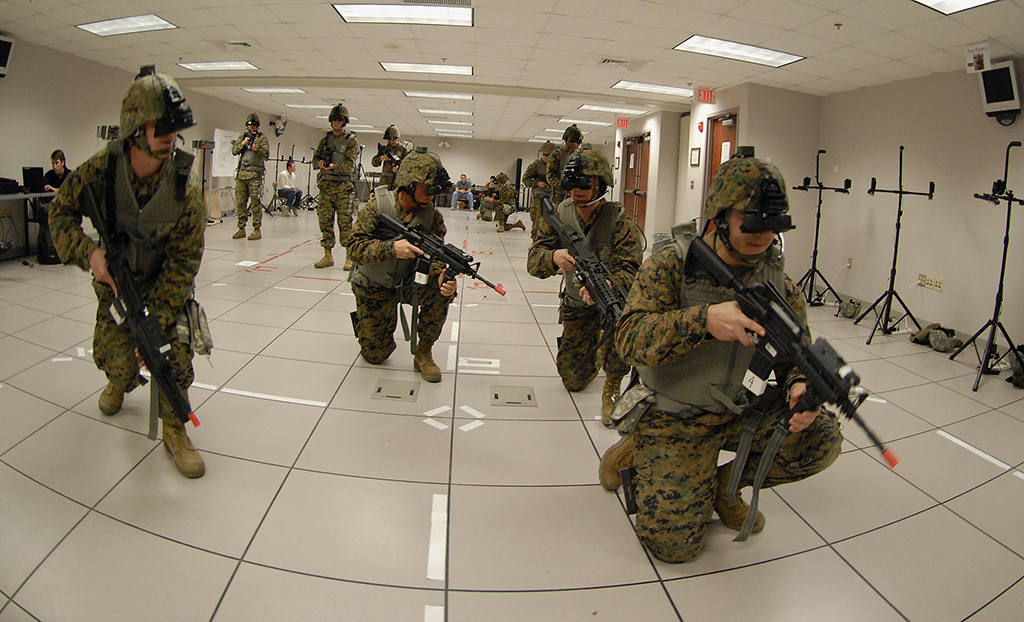
\includegraphics[width=10cm]{imagenes/vr_military}
	\caption{Marines de los Estados Unidos entrenando con el FITE (\textit{Future Immersive Training Environment}), un sistema de entrenamiento VR}
	\label{fig:vr_military}
\end{figure}

La verdadera importancia y utilidad de esto se muestra de dos formas muy claras: \textbf{facilidad de acceso}, requiriendo una serie de equipos mucho más al alcance y masificable; y \textbf{ahorro de recursos}, como podría ser el combustible de avión o la munición \cite{costeffective_vr}.

\subsection{Evolución y estado actual}

De hecho, la realidad virtual nunca había sido algo que se tuviese muy en cuenta a un nivel tecnológico hasta los últimos años, únicamente formando parte en conversaciones sobre futuros idílicos \cite{innovation_vr}. En la última década, en cambio, la evolución del hardware ha sido espectacular.

Las primeras gafas de realidad virtual como las conocemos ahora fueron el primer kit de desarrollo de Oculus, el cual tenía una resolución de 640x800 píxeles en cada ojo. A día de hoy, esta resolución ha llegado a cuadriplicarse (Figura \ref{fig:vr_resolution}). Además de resolución, otras muchas características también han avanzado, como el ángulo de visión, la tasa de refresco, uso inalámbrico, etcétera.

Aparte de las propias gafas, otros elementos físicos han tenido una evolución drástica, como por ejemplo mandos con una mayor optimización del uso de su batería o con seguimiento de posición de los dedos \cite{fingertracking}, nodos de seguimiento para colocar en diferentes puntos del cuerpo y capturar el movimiento de este, cámaras de captura de movimiento de la cara, y otros muchos elementos modulares que mejoran y amplían el uso de la realidad virtual.

\begin{figure}[H]
	\centering
	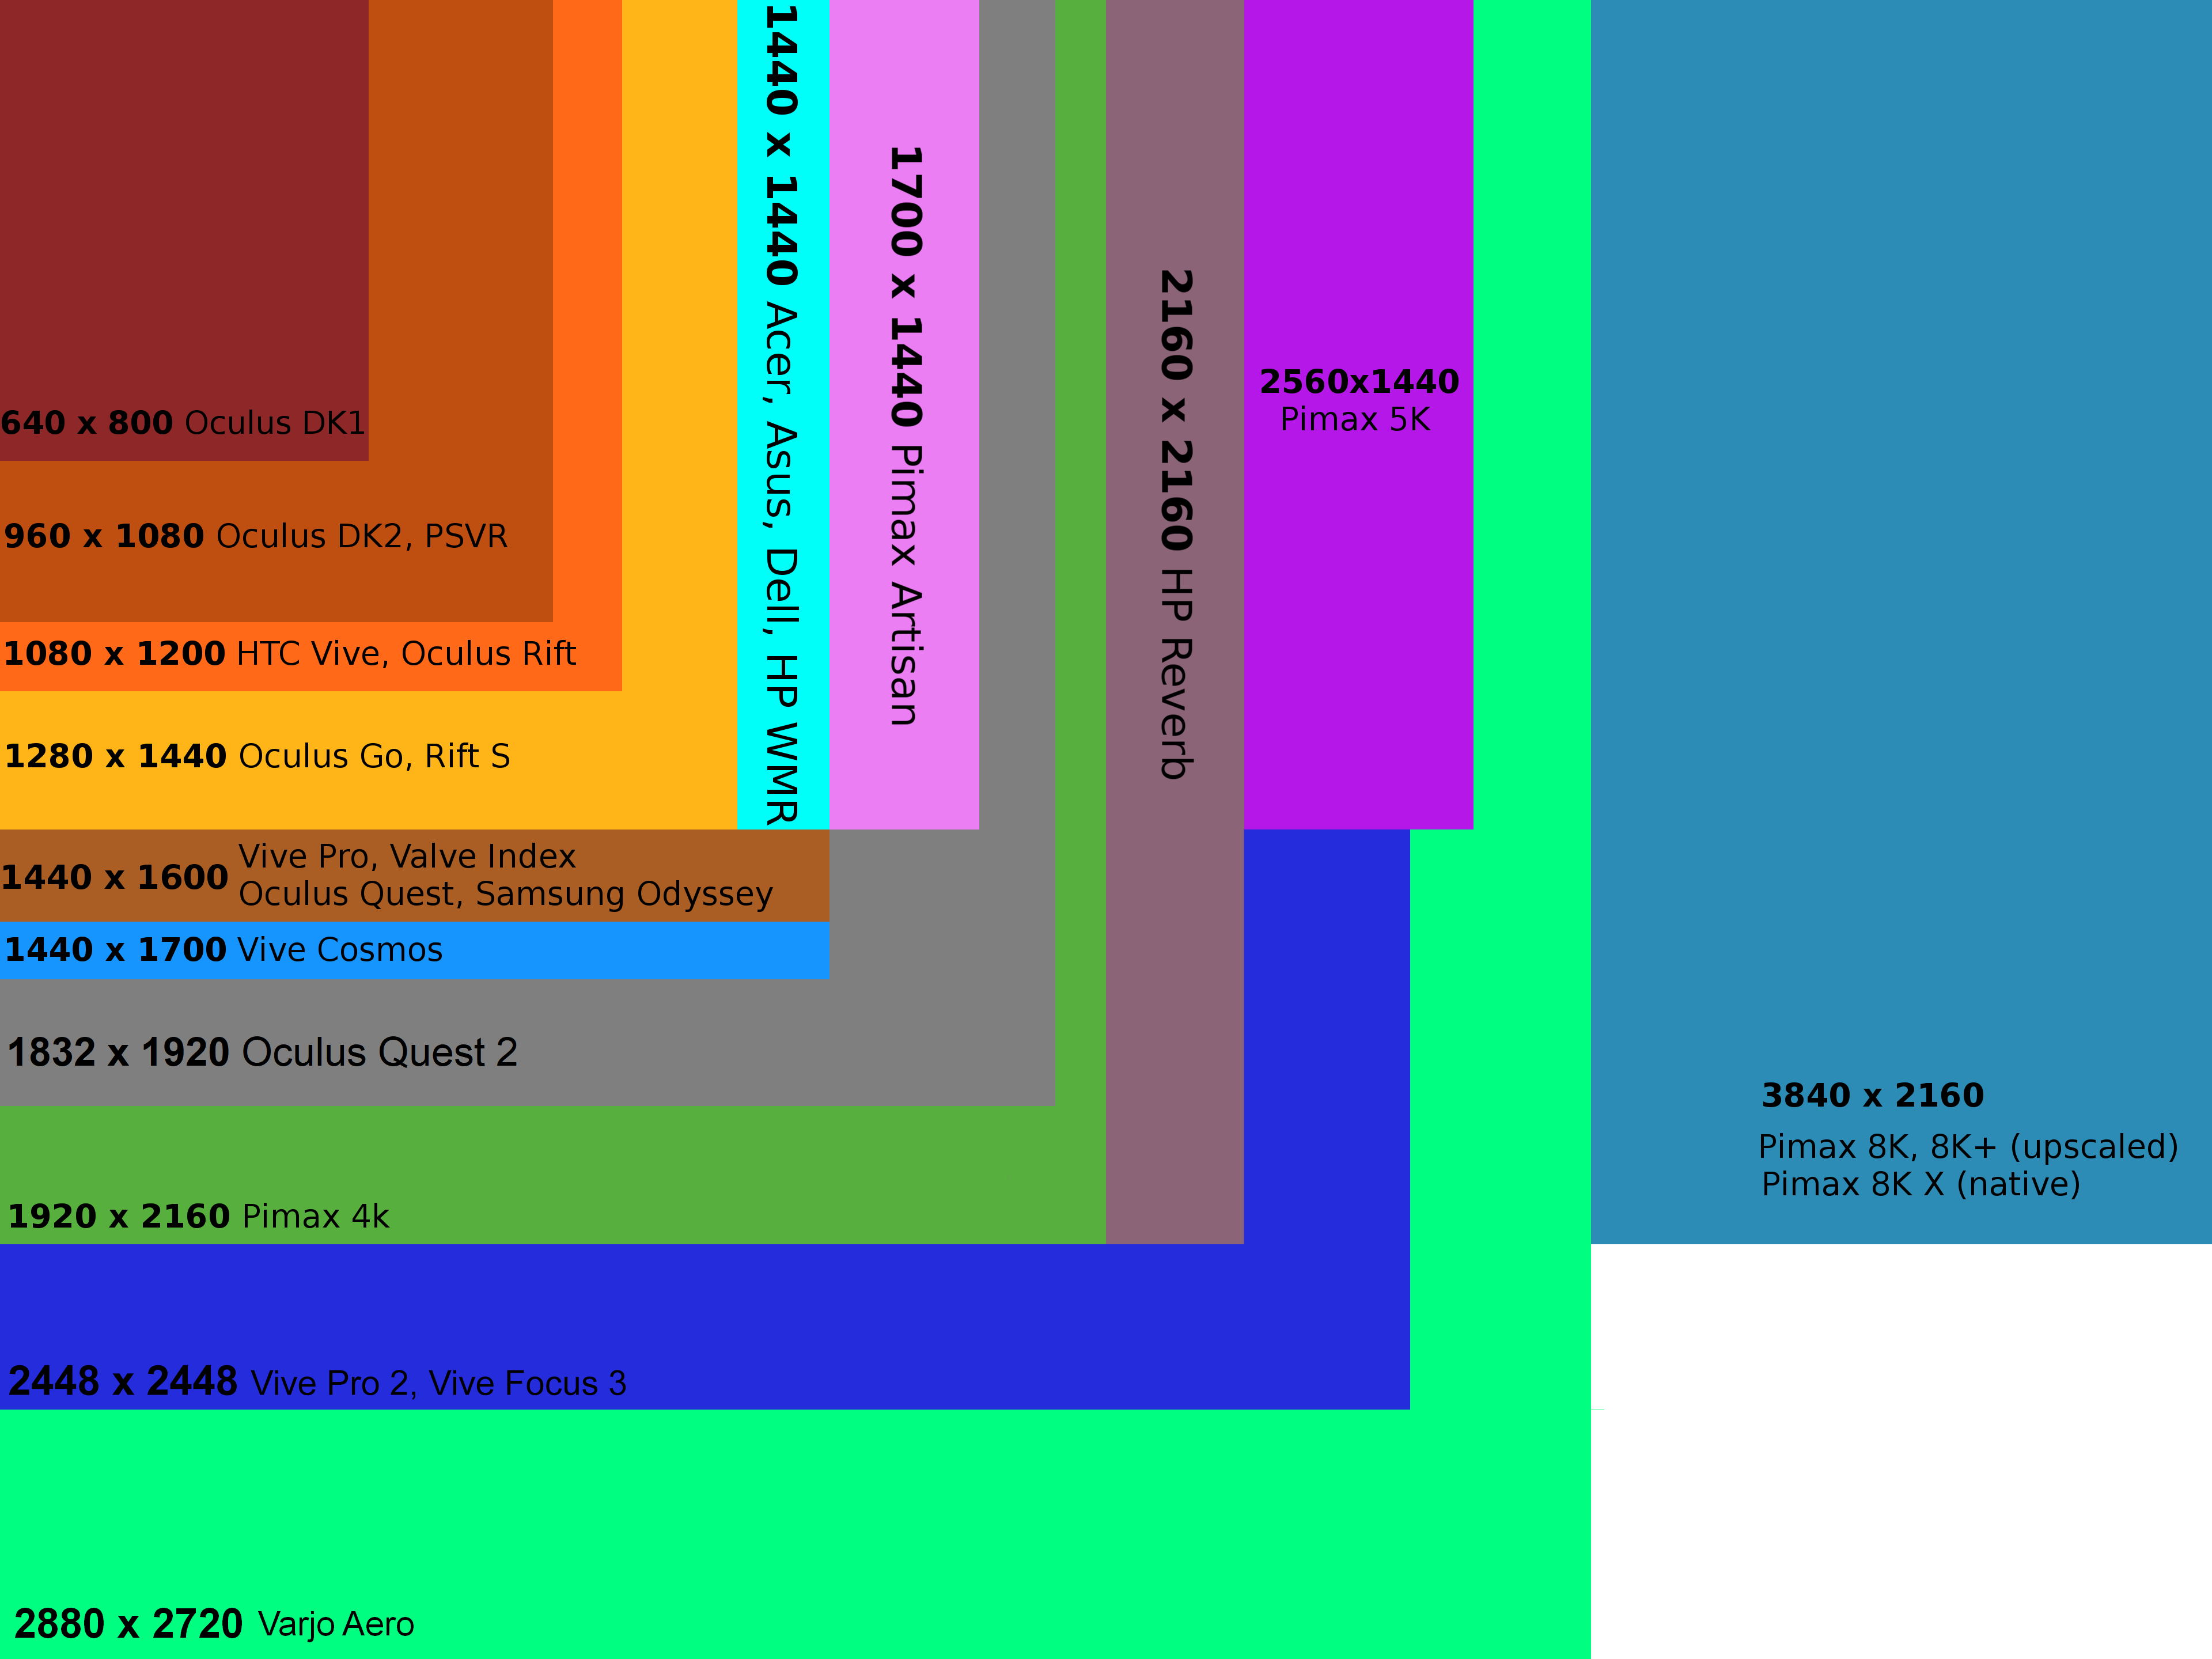
\includegraphics[width=10cm]{imagenes/vr_resolution}
	\caption{Tabla comparativa de la resolución por ojo de las gafas de realidad virtual más conocidas}
	\label{fig:vr_resolution}
\end{figure}

Además de simples mejoras físicas, la realidad virtual también se ha beneficiado de un gran \textbf{crecimiento en su comunidad}, tanto consumidores como desarrolladores de todo tipo debido a unas prestaciones cada vez más interesantes, lo que a su vez lleva a una mayor cantidad de productos, tanto software como hardware, junto a la demanda de estos \cite{vr_evolution}.

En lo que al desarrollo de aplicaciones respecta, las más avanzadas han sido creadas usando el motor gráfico \textbf{Unreal Engine 5} debido, entre otras razones, a su alto rendimiento y numerosas herramientas para el desarrollo de realidad virtual. Es por esto que se ha elegido para el proyecto en mano.

\section{Unreal}

Como ya se ha mencionado, Unreal es de los motores gráficos 3D más usados para el desarrollo de aplicaciones de realidad virtual, en concreto para las más especializadas. Esto se debe, entre otros factores, a las herramientas avanzadas que permiten aplicaciones imposibles de desarrollar en otros motores, además de un proceso más simplificado frente a estos \cite{unreal}.

En concreto, una biblioteca de Unreal lanzada recientemente, la cual permite \textbf{modificar la forma y colisión de los modelos en tiempo de ejecución a través de operaciones booleanas}, será clave en el desarrollo del proyecto, siendo la falta de una herramienta parecida la razón de que no existiese ninguna aplicación parecida hasta el momento.

\section{Escultura en mármol}

\subsection{Historia y características}

La escultura es uno de los artes más antiguos que existen, y en concreto, el mármol es de los materiales más usados para este. \textit{Venus de Milo} (100 a. C.), \textit{Laocoonte y sus hijos} (siglo I d. C.) (Figura \ref{fig:laocoonte_escultura}) o el \textit{David de Miguel Ángel} (1501-4 d. C.) son solo algunas de las obras más famosas esculpidas con esta técnica.

\begin{figure}[H]
	\centering
	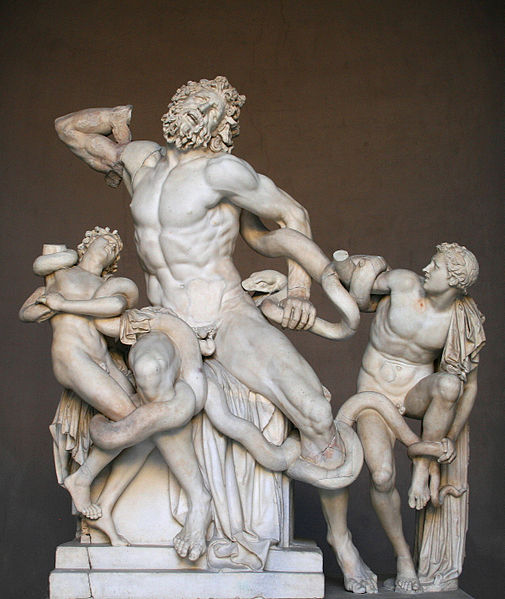
\includegraphics[width=6.5cm]{imagenes/laocoonte_escultura}
	\caption{\textit{Laocoonte y sus hijos}, también conocido como el Grupo del Laocoonte. Mármol copia de un original helenístico del 200 aC aproximadamente. Procedencia: Termas de Trajano, a principios de 1507.}
	\label{fig:laocoonte_escultura}
\end{figure}

El uso de mármol para la escultura se remonta a la Edad Antigua, y se ha utilizado tanto para relieves como para estatuaria. Desde entonces, ha sido un material apreciado por artistas debido a sus propiedades:

\begin{itemize}
	\item Fácil de trabajar y suave cuando se extrae.
	\item Adquiere dureza con la edad, lo que le da resistencia a la figura acabada.
	\item Variedad de tonos y patrones.
	\item Bajo índice de refracción de la luz, como la piel humana, lo que permite una apariencia humana.
	\item Grano más fino en comparación a otras piedras, lo que permite presentar detalles minuciosos.
\end{itemize}

Sin embargo, también existen una serie de inconvenientes. El mármol es muy pesado, más que otras piedras, además de más caro que estas. Otro inconveniente es que es más vulnerable a agrietarse que otros materiales como el bronce. También es menos resistente al clima que otras piedras como el granito, y absorbe con facilidad aceites como los de la piel, lo que puede causar manchas. \cite{sculpture_introduction}.

\subsection{Herramientas y técnicas}

Aunque se puede empezar la talla de forma directa, lo normal es esquematizar previamente la escultura a través de bocetos, tanto en dibujo como tallando versiones en miniatura con materiales baratos, para luego usarlos como guía para la figura final.

Una vez iniciado el proceso, se necesita una serie de herramientas para trabajar. Estas herramientas, aunque se han adaptado y mejorado a lo largo de la historia, son esencialmente las mismas, con el uso ocasional de utensilios más modernos para facilitar el proceso:

\begin{itemize}
	\item \textbf{Cincel}: La herramienta más importante en la escultura. Existen distintos tipos.
	\begin{itemize}
		\item \textbf{En punta}: Usado para quitar gran cantidad de material de un solo golpe, lo que permite llegar antes a la parte del mármol que conformará la propia escultura posteriormente. También existen cinceles de punta ancha con el mismo propósito.
		\item \textbf{De dientes}: Con múltiples dientes en la punta, que crean líneas paralelas. Se usa principalmente para refinar la forma dejada por el cincel en punta, eliminando irregularidades en la figura y permitiendo mayor comodidad y precisión al continuar.
		\item \textbf{Plano}: Como el nombre indica, la punta es plana, y sirve para tallar los detalles.
		\item \textbf{Redondo}: Lo mismo que el plano, pero con otro resultado en la textura.
	\end{itemize}
	\item \textbf{Martillo}: Con el que se golpea la parte roma del cincel para que la fuerza del golpe se concentre en la punta.
	\item \textbf{Bujarda}: Martillo con la cabeza recubierta de dientes. Se golpea directamente a la piedra con él para dejar formas rugosas.
	\item \textbf{Martillo neumático}: Martillo con mecanismo neumático para golpear reiteradas veces en un mismo punto. Se usa para lo mismo que el cincel en punta.
	\item \textbf{Radial}: Se usa para cavar líneas rectas de forma rápida. Una forma común, rápida y efectiva de quitar material inicial es hacer cortes paralelos con una radial para quitar el sobrante con martillo y cincel.
	\item \textbf{Limas, lijas, piedra pómez y otras}: Cualquier herramienta que sirva para pulir el resultado final.
\end{itemize}

Con todas estas herramientas se puede proceder a trabajar la piedra. Primero, se desbasta el material, es decir, se elimina todo el material muy exterior a lo necesario. Para esto se puede usar la radial, el martillo neumático o simplemente el cincel en punta. Conforme se progresa la tarea, se pasa a herramientas como el cincel de dientes para obtener la forma cruda de la escultura final, a la que luego se le añaden todos los detalles poco a poco con los cinceles planos y/o redondos. Finalmente, se pule y se limpia \cite{marble_techniques}.

\subsection{Complejidad y coste}

Como es de esperar, esta no es una práctica ni sencilla ni accesible. Acceso a todos los materiales, herramientas, espacio adaptado y necesario son algunos de los elementos necesarios para esculpir mármol. Además, mucha práctica e intentos fallidos son necesarios antes de obtener buenos resultados, lo cual puede llegar a ser muy frustrante, sobretodo cuando hace falta invertir tanto para siquiera iniciarse en el arte.

\section{Trabajos previos}

Existen muchas aplicaciones de realidad virtual que simulan prácticas del mundo real, ya sea de forma más ludificada y poco realista, como \textit{Cooking Simulator VR} (2021), o lo más cercano posible a la realidad, como el simulador de conducción \textit{Assetto Corsa} (2014), usado incluso por pilotos de carreras profesionales.

Por supuesto, también existen multitud de herramientas creativas que permiten dibujar, animar y, por supuesto, modelar en realidad virtual. \textit{SculptrVR} (2016) (Figura \ref{fig:sculptrvr}) o \textit{AnimVR} (2018) son algunos de los ejemplos de este tipo de aplicaciones, que permiten crear modelos en 3D o rodar películas de animación, respectivamente.

\setcounter{footnote}{0}

\begin{figure}[H]
	\centering
	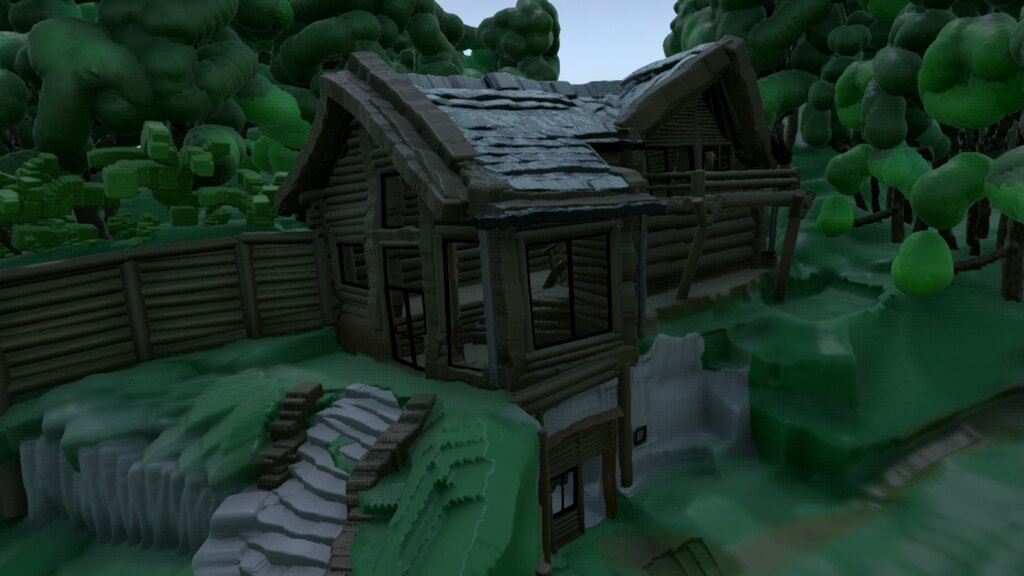
\includegraphics[width=10cm]{imagenes/sculptrvr}
	\caption[Captura de pantalla de una escena realizada en \textit{SculptrVR} por el usuario  topgunsi en Steam]{Captura de pantalla de una escena realizada en \textit{SculptrVR} por el usuario  topgunsi\protect\footnotemark[1]{} en Steam}
	\label{fig:sculptrvr}
\end{figure}

\footnotetext[1]{\url{https://steamcommunity.com/sharedfiles/filedetails/?id=1267529147}}

Sin embargo, generalmente, este tipo de aplicaciones no tratan de simular la realidad, sino que buscan \textbf{permitir formas de creatividad que no serían posibles fuera del mundo virtual}, como por ejemplo, dibujando objetos 3D en el aire.

\section{Motivación}

Por esta misma razón, la idea es desarrollar ChiselVR, un software para realidad virtual en el que, en lugar de crear esculturas a través de la adición como otras aplicaciones de modelaje, se crearían a través de \textbf{sustracción}, imitando el proceso de esculpir en mármol con sus correspondientes herramientas.

Por supuesto, esta es una forma más lenta y menos vistosa de modelar que la que ofrecen las demás aplicaciones, pero lo interesante reside en eso: \textbf{imitar la realidad} y permitir al usuario experimentar el proceso de esculpir de la forma tradicional sin tener que invertir en todo el material necesario para ello.

La aplicación final ofrecerá al usuario la posibilidad de iniciar un proyecto con un bloque de mármol que podrá esculpir a voluntad con las herramientas necesarias y esperadas para ello.